\documentclass[usenames,dvipsnames]{beamer}
%
% Choose how your presentation looks.
%
% For more themes, color themes and font themes, see:
% http://deic.uab.es/~iblanes/beamer_gallery/index_by_theme.html
%
\mode<presentation>
{
  \usetheme{default}      % or try Darmstadt, Madrid, Warsaw, ...
  \usecolortheme{default} % or try albatross, beaver, crane, ...
  \usefonttheme{default}  % or try serif, structurebold, ...
  \setbeamertemplate{navigation symbols}{}
  \setbeamertemplate{caption}[numbered]
} 

\usepackage[francais]{babel}
\usepackage[utf8]{inputenc}
\usepackage[T1]{fontenc}
\usetheme{Boadilla}
\usepackage{amsmath}

\usepackage[backend=biber,style=authoryear-comp,uniquename=init,firstinits=true,
            %% "et al" pour > deux auteurs, & pour exactement 2
            uniquelist=false,maxcitenames=2,mincitenames=1,maxbibnames=99,
            isbn=false,url=false,doi=false
]{biblatex}


\renewcommand{\cite}{\parencite}
\renewcommand*{\nameyeardelim}{\addcomma \addnbspace}
\renewcommand*{\revsdnamedelim}{}
\renewcommand*\finalnamedelim{ \& }

\DefineBibliographyExtras{french}{\restorecommand\mkbibnamelast}

\DeclareNameAlias{default}{last-first}
\DeclareNameAlias{sortname}{last-first}

% Supprimer les guillemets dans les titres
\DeclareFieldFormat[article,incollection,unpublished,inproceedings]{title}{#1}

% Je n'aime pas, mais j'ai l'impression que mlapafr utilise ça
\renewbibmacro{in:}{\printtext{In} \addspace}


% Espaces insécables dans les citations et la bibliographie (noms de
% conférences) ?

\usepackage{xpatch}
\usepackage{xstring}
%\xpatchbibmacro{series+number}{\addspace}{\addnbspace}{}{}

\renewbibmacro*{series+number}{%
  \setunit*{\addnbspace}%
  \printfield{series}%
  \printfield{number}%
  \newunit}

\newcommand{\beamcite}[1]{\hfill {\footnotesize \textcite{#1}}}
\newcommand{\red}[1]{\textcolor{red}{#1}}
\newcommand{\magenta}[1]{\textcolor{magenta}{#1}}
\newcommand{\blue}[1]{\textcolor{blue}{#1}}

%%%%%%%%%%%%%%%%%%%%%%%%


\addbibresource{references.bib}


\title[Classification monotone]{Apprentissage et classification monotone}
\author{Laura Nguyen}
\institute{LFI}
\date{19 juillet 2018}

\newcommand{\myfrac}[2]{\frac{\displaystyle {#1}}{\displaystyle {#2}}}

\begin{document}

\begin{frame}
  \titlepage
\end{frame}

% Uncomment these lines for an automatically generated outline.
%\begin{frame}{Outline}
%  \tableofcontents
%\end{frame}

\section{Introduction}

\begin{frame}{Classification monotone}
\begin{itemize}
\item Classifieur monotone :
    \begin{itemize}
        \item Exploiter la monotonie de la classe par rapport aux attributs
        \item Classifieur aussi monotone que possible et maintenant de bonnes performances
    \end{itemize}
\item Concepts sémantiques : préférence, priorité, importance...
\item Applications : 
    \begin{itemize}
        \item Prédiction du risque de faillite
        \item Evaluation du prix de biens immobiliers
        \item Cote de crédit 
    \end{itemize}
\item \textcite{pazzani-acceptance} :
    \begin{itemize}
        \item Etude auprès des experts (médecins)
        \item Gain d'interprétabilité
        \item Performances équivalentes 
    \end{itemize}
\end{itemize}
\end{frame}

\begin{frame}{Exemple de problème de classification monotone}
\textcite{potharst-classification-bank}

\begin{table}
\resizebox{\textwidth}{!}{
\begin{tabular}{|*{4}{c|} | c |}
    \hline
        client & revenu & éducation & casier judiciaire & prêt \\
    \hline 
        cl1 & faible & faible & juste & non\\
        cl2 & faible & faible & excellent & faible\\
        cl3 & moyen & intermédiaire & excellent & intermédiaire\\
        cl4 & élevé & faible & excellent & élevé\\
        cl5 & élevé & intermédiaire & excellent & élevé\\
    \hline
\end{tabular}}
\label{tab:bank-loan-dataset}
\end{table}

\end{frame}

\begin{frame}{Formalisation}

\begin{itemize}
\item Entrées :  
\begin{itemize}
	\item n exemples : $\Omega = \{\omega_1, ... , \omega_n\}$
    \item m attributs ordonnés : $A = \{a_1, ... , a_m\}$. \\ Pour $j=1,... ,m :$
    	\begin{itemize}
    	\item $a_j : \Omega \rightarrow X_j$ avec $X_j$ totalement ordonné
        \item Espace de description $X = X_1 \times ... \times X_m$
    	\end{itemize}
    \item k classes : $C = \{c_1, ... , c_k\}$
\end{itemize}
\item Sortie : 
\begin{itemize}
\item Fonction de classification monotone $\lambda : X \rightarrow C$
\end{itemize}
\end{itemize}

\end{frame}

\begin{frame}{Dataset artificiel à un attribut monotone}

\begin{figure}
	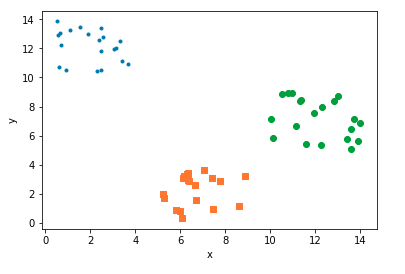
\includegraphics[width=.7\textwidth]{artificial-dataset.png}
\end{figure}

\end{frame}

\begin{frame}{Classification par arbres de décision}
\begin{itemize}
\item Pas d'hypothèse sur les données
%\item Exploiter au mieux l'éventuelle gradualité entre les valeurs d'attributs et la classe
\item Construction :
\begin{itemize}
\item Choisir $a_j$ respectant le plus la contrainte de monotonie locale: \\~\

$$\forall \omega_i, \omega_h \in \Omega, a_j(\omega_i) \leq a_j(\omega_h) \Rightarrow \lambda(\omega_i) \leq \lambda(\omega_h)$$ \\~\

\item Approche gloutonne : pas de garantie d'avoir un classifieur globalement monotone

\end{itemize}
\end{itemize}

\end{frame}

\begin{frame}{Mesures de discrimination monotone}
    \begin{itemize}
    \item Problème : incapacité des mesures de discrimination classiques à détecter la monotonie 
    \item Chercher des mesures de discrimination sensibles à la monotonie et robustes au bruit non-monotone
    \begin{itemize}
        \item Généralisation à rang de mesures classiques (Shannon, Gini)
        \item Modèle de construction hiérarchique
        \item Nouvelles mesures
    \end{itemize}
\end{itemize}
\end{frame}

\begin{frame}{Ensembles dominants}
Pour $\omega_i \in \Omega,$
\begin{itemize}
\item Classes d'équivalence générées par : 
\begin{itemize}
\item un attribut $a_j$ : $$[\omega_i]_{a_j} = \{\omega_h \in \Omega : a_j(\omega_i) = a_j(\omega_h)\}$$
\item la classe $\lambda$ : $$[\omega_i]_{\lambda} = \{\omega_h \in \Omega : \lambda(\omega_i) = \lambda(\omega_h)\}$$
\end{itemize}

\item Ensembles dominants générés par :
\begin{itemize}
\item un attribut $a_j$ : $$[\omega_i]^{\leq}_{a_j} = \{\omega_h \in \Omega : a_j(\omega_i) \leq a_j(\omega_h)\}$$
\item la classe $\lambda$ : $$[\omega_i]^{\leq}_{\lambda} = \{\omega_h \in \Omega : \lambda(\omega_i) \leq \lambda(\omega_h)\}$$
\end{itemize}

\end{itemize}
\end{frame}

%\begin{frame}{Ensembles dominants : exemple}
%Soit le dataset suivant :
%
%\begin{table}
%\begin{tabular}{|*{3}{c|} | c |}
%    \hline
%        $\Omega$ & $a_1$ & $a_2$ & $\lambda$ \\
%    \hline 
%        $\omega_1$ & 1 & 5 & 1 \\ 
%        $\omega_2$ & 1 & 7 & 1 \\
%        $\omega_3$ & 2 & 8 & 1\\
%        $\omega_4$ & 5 & 9 & 2 \\
%        $\omega_5$ & 5 & 7 & 2 \\ 
%        $\omega_6$ & 4  & 6 & 2\\
%    \hline
%\end{tabular}
%
%\begin{itemize}
%    \item L'ensemble dominant généré par $a_1$ pour $\omega_3$ est : 
%        $$[\omega_3]^{\leq}_{a_1} = \{\omega_3, \omega_4, \omega_5, \omega_6\}$$
%    \item L'ensemble dominant généré par $\lambda$ pour $\omega_3$ est :
%        $$[\omega_3]^{\leq}_{\lambda} = \{\omega_1, \omega_2, \omega_3, \omega_4, \omega_5, \omega_6\}$$
%\end{itemize}
%
%\label{tab:dsa-dataset}
%
%
%
%\end{table}
%
%
%\end{frame}

\begin{frame}{Généralisation à rang de l'entropie de Shannon \beamcite{hu-information}}
\begin{itemize}
\item Entropie conditionnelle de Shannon: 
    \begin{align*}
        H_s\left(\lambda | a_j\right) &= \sum_{s=1}^{t_j}p_s\left(-\sum_{q=1}^{k}\myfrac{p_{q,s}}{p_s}\log\left(\myfrac{p_{q,s}}{p_s}\right)\right)\\
            &= \sum_{i=1}^{|\Omega|} \frac{1}{|\Omega|}\left(\log \left(\frac{|[\omega_i]_{\lambda} \cap [\omega_i]_{a_j}|}{|[\omega_i]_{a_j}|}\right)\right)
    \end{align*}
\item Entropie de Shannon d'ordre: 

    $$H^*_s\left(\lambda | a_j\right) = \sum_{i=1}^{|\Omega|} \frac{1}{|\Omega|}\left(\log \left(\frac{|[\omega_i]^{\leq}_{\lambda} \cap [\omega_i]^{\leq}_{a_j}|}{|[\omega_i]^{\leq}_{a_j}|}\right)\right)$$

\end{itemize}

\end{frame}

\begin{frame}{Modèle de construction hiérarchique de mesures de discrimination à rang \beamcite{marsala-rank}}
\begin{itemize}
\item Isoler les propriétés d'une telle mesure
\item Créer de nouvelles mesures
\item Structure fonctionnelle commune avec 3 fonctions \\
Pour $a_j$ fixé :
\begin{itemize}
\item $f^*$ : mesure de monotonie locale de l'objet
\item $g^*$ : mesure d'agrégation de $f^*$
\item $h^*$ : agrégation de mesures $g^*$
\end{itemize}
Ecriture générique : \\~\
            $$H^*(\lambda | a_j) = h^*(g^*(f^*(\omega_1)),...,g^*(f^*(\omega_n)))$$
\end{itemize}
\end{frame}


\begin{frame}{Couche $f^*$}
    Pour $a_j \in A$ fixé,
    \begin{itemize}
        \item $dsr(\omega_i) = \myfrac{| [\omega_i]^{\leq}_{\lambda} \cap [\omega_i]^{\leq}_{a_j}|}{| [\omega_i]^{\leq}_{a_j} |}$
        \item $mindsr(\omega_i) = \myfrac{min_{\omega_h \in [\omega_i]_{a_j}} |[\omega_h]^{\leq}_{\lambda} \cap [\omega_h]^{\leq}_{a_j}|}{| [\omega_i]^{\leq}_{a_j} |}$
        \item $maxdsr(\omega_i) = \myfrac{max_{\omega_h \in [\omega_i]_{a_j}} |[\omega_h]^{\leq}_{\lambda} \cap [\omega_h]^{\leq}_{a_j}|}{| [\omega_i]^{\leq}_{a_j} |}$
        \item $avgdsr(\omega_i) = \myfrac{\displaystyle\sum_{\omega_h \in [\omega_i]_{a_j}} \myfrac{|[\omega_h]^{\leq}_{\lambda} \cap [\omega_h]^{\leq}_{a_j}|}{|[\omega_i]_{a_j}|}}{| [\omega_i]^{\leq}_{a_j} |}$
    \end{itemize}
\end{frame}

\begin{frame}{Réécriture des mesures de discrimination à rang}
         $$H^*_S\left(\lambda|a_j\right) = \displaystyle\sum_{i=1}^{n}\myfrac{1}{n} \left(-\log\left(dsr\left(\omega_i\right)\right)\right)$$
        \begin{itemize}
            \item $f^*_S : dsr(\omega_i)$
            \item $g^*_S : -\log(f^*_S(\omega_i))$
            \item $h^*_S : \sum_{i=1}^{n} \myfrac{1}{n} g^*_S(f^*_S(\omega_i))$
        \end{itemize}
     $$H^*_P\left(\lambda|a_j\right) = \displaystyle\sum_{i=1}^{n}\myfrac{1}{n} \left(-\myfrac{\log\left(mindsr\left(\omega_i\right)\right)}{mindsr\left(\omega_i\right)}\right)$$
        \begin{itemize}
            \item $f^*_P : mindsr(\omega_i)$
            \item $g^*_P : -\myfrac{\log f^*_P(\omega_i)}{f^*_P(\omega_i)}$
            \item $h^*_P : \sum_{i=1}^{n} \myfrac{1}{n} g^*_P(f^*_P(\omega_i))$
        \end{itemize}
\end{frame}

\begin{frame}{Construction d'arbres de décision monotones \beamcite{marsala-rank}}
    \begin{itemize}
        \item Classifieur RDMT(H) paramétré par : 
            \begin{itemize}
                \item Une mesure de discrimination H
                \item 3 critères : partitionnement, arrêt, étiquetage
            \end{itemize}
        \item Critère de partitionnement (splitting rule)
            \begin{itemize}
                \item Chaque attribut $a_j$ est binarisé : $\forall x \in X_j$,
                    \begin{equation*}
                    \begin{array}{cl}
                        a^x_j(\omega_i) = \begin{cases}{0} &\text{ si } a_j(\omega_i) \leq x\\
                          {1} &\text{sinon}\end{cases}
                     \end{array}
                     \end{equation*}
                \item Trouver $a^{x_*}_*$ minimisant $H(\lambda|a^x_j)$
                    \begin{itemize}
                        \item $a_*$ est l'attribut utilisé pour le partitionnement
                        \item $x_*$ est la valeur seuil trouvée par discrétisation: 
                            \begin{equation*}
                            \begin{array}{cl}
                                x_* = arg\,min \{H(\lambda|a^x_j) | j=1,...,m, x \in X_j\}
                            \end{array}
                            \end{equation*}
                    \end{itemize}
            \end{itemize}
    \end{itemize}
\end{frame}

\begin{frame}{Critère de partitionnement}
    \begin{columns}
        \begin{column}{0.5\textwidth}
            \centering
            Seuil de coupure généré par $H^*_S$ : \\
            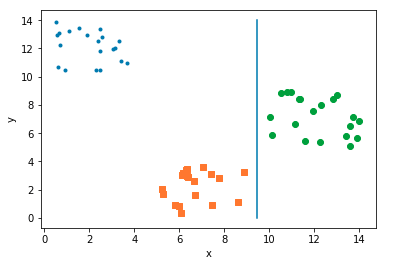
\includegraphics[width=0.8\textwidth]{threshold_rsdm.png}
            $$H^*_S(\lambda | x) =  0.19 \leq H^*_S(\lambda | y) =  0.53$$
        \end{column}
        \begin{column}{0.5\textwidth}
            \centering
            Seuil de coupure généré par $H_S$ :
	    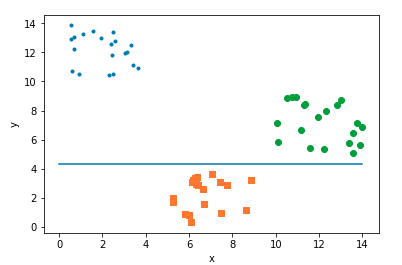
\includegraphics[width=0.8\textwidth]{threshold_sdm.png}
        $$H_S(\lambda | x) = H_S(\lambda | y) =  0.67$$
        \end{column}
    \end{columns}
\end{frame}

\begin{frame}{Arbres de décision générés par $H^*_S$ et $H_S$}
    \begin{figure}
    	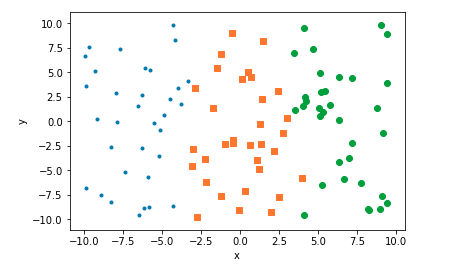
\includegraphics[width=.35\textwidth]{Capture_d__cran_de_2018-07-11_20-06-25.png}
    \end{figure}
    \begin{columns}
        \begin{column}{0.45\textwidth}
            \centering
            Arbre généré par $H^*_S$\\
            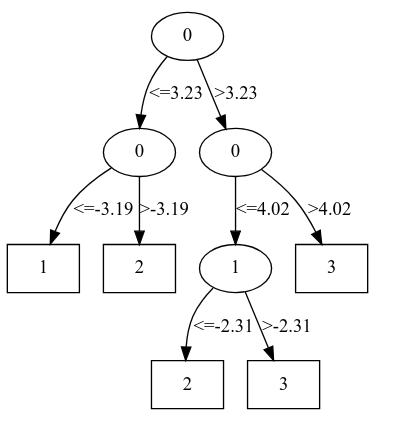
\includegraphics[width=0.5\textwidth]{rsdm-tree-artificial.png}
            \vspace*{2.5cm}
        \end{column}
        \begin{column}{0.45\textwidth}
            \centering
            Arbre généré par $H_S$
	    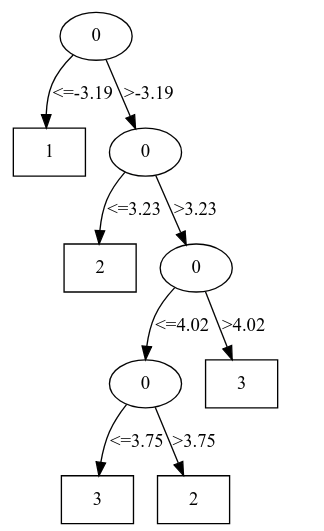
\includegraphics[width=0.5\textwidth]{sdm-tree-artificial.png}
        \end{column}
    \end{columns}
\end{frame}

\begin{frame}{Expérimentations sur des datasets jouets}
    \begin{columns}
        \begin{column}{0.45\textwidth}
            \centering
            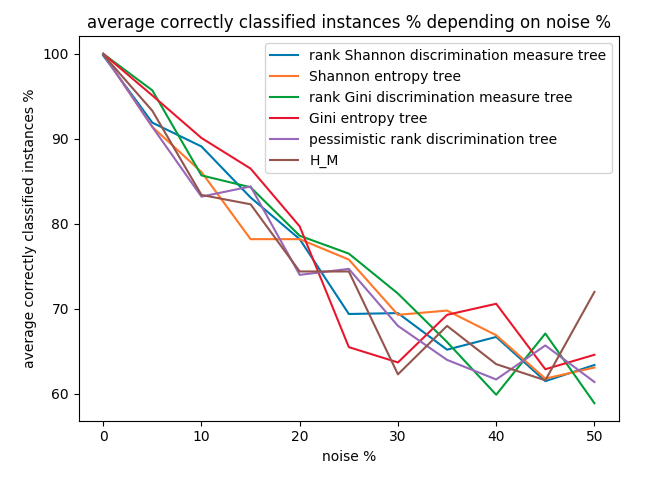
\includegraphics[width=\textwidth]{acc_2.png}
        \end{column}
        \begin{column}{0.45\textwidth}
            \centering
            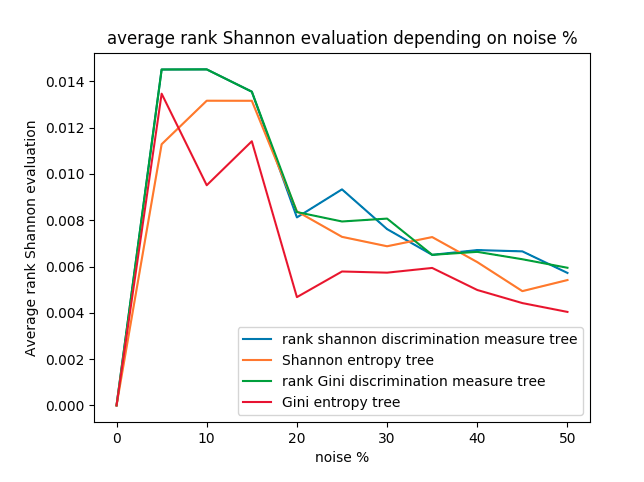
\includegraphics[width=\textwidth]{shannon_eval_2.png}
        \end{column}
    \end{columns}
    \begin{columns}
        \begin{column}{0.45\textwidth}
            \centering
            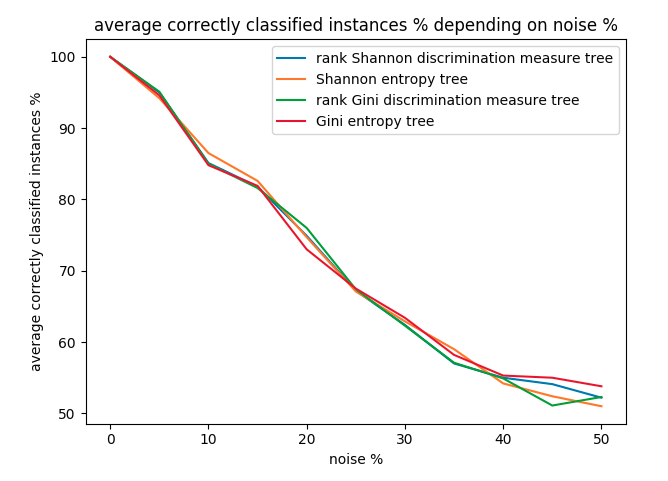
\includegraphics[width=\textwidth]{acc_3.png}
        \end{column}
        \begin{column}{0.45\textwidth}
            \centering
            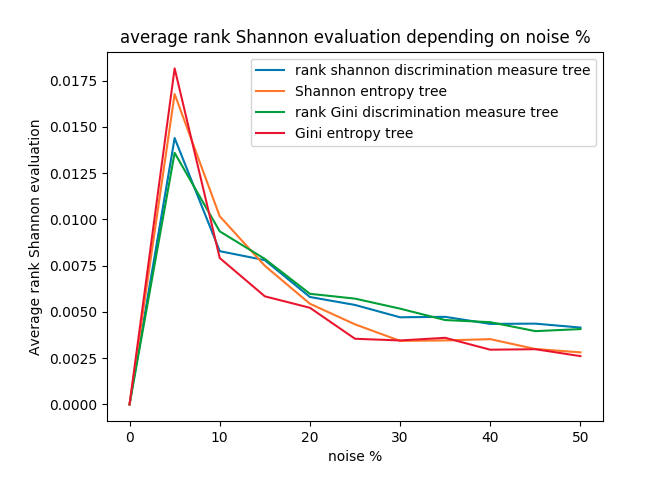
\includegraphics[width=\textwidth]{shannon_eval_3.png}
        \end{column}
    \end{columns}
\end{frame}

\begin{frame}{Expérimentations sur des datasets jouets}
    \begin{columns}
        \begin{column}{0.5\textwidth}
            \centering
            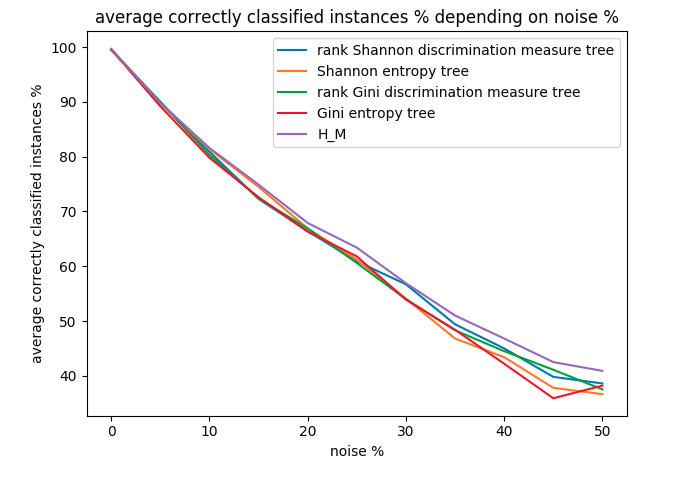
\includegraphics[width=\textwidth]{acc_5.png}
        \end{column}
        \begin{column}{0.5\textwidth}
            \centering
            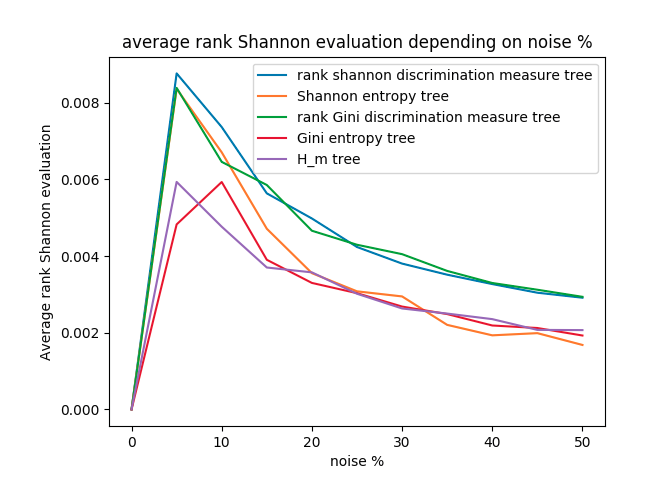
\includegraphics[width=\textwidth]{shannon_eval_5.png}
        \end{column}
    \end{columns}
\end{frame}

\begin{frame}{Expérimentations sur des datasets jouets : ratio du nombre de paires d'éléments non monotones}
    \begin{columns}
        \begin{column}{0.45\textwidth}
            \centering
            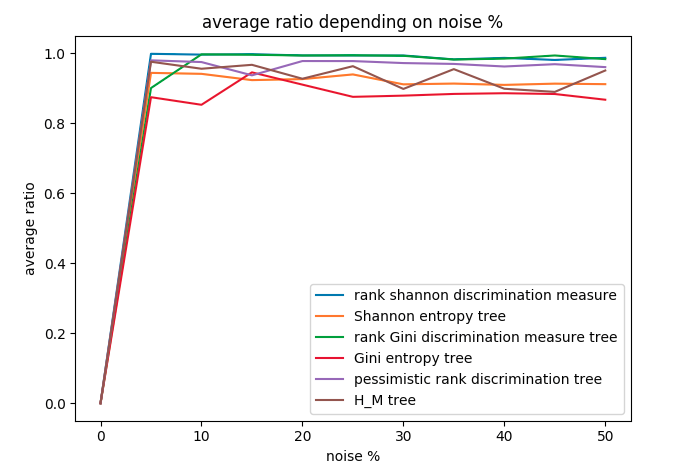
\includegraphics[width=\textwidth]{ratio_2.png}
        \end{column}
        \begin{column}{0.45\textwidth}
            \centering
            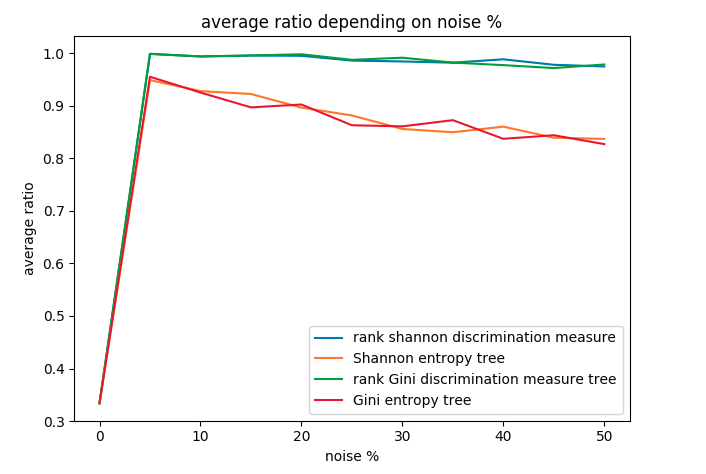
\includegraphics[width=\textwidth]{ratio_3.png}
        \end{column}
    \end{columns}
    \begin{columns}
        \begin{column}{0.45\textwidth}
            \centering
            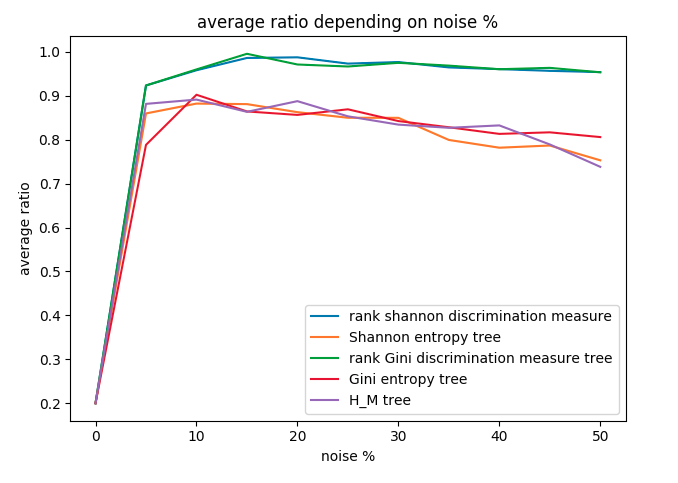
\includegraphics[width=\textwidth]{ratio_5.png}
        \end{column}
    \end{columns}

\end{frame}

\begin{frame}{Expérimentations sur des datasets artificiels}

    \begin{itemize}
        \item CPU (classification) : 8 classes, 9 attributs, 209 instances
        \begin{table}
            \resizebox{0.8\textwidth}{!}{
            \begin{tabular}{|*{4}{c|}}
                \hline
                   & $H^{*}_S$  & $H_S$ & $H^{*}_Q$ \\
                \hline
                CCI  & 68.40 \% $\pm$ 0.04 \% & 65.06 \% $\pm$ 0.03 \%  & 67.93 \% $\pm$ 0.03 \%  \\
                avgDepth  & 10.50 $\pm$ 0.50& 9.00 $\pm$ 0.00& 11.00 $\pm$ 1.00 \\
                avgLeaves  & 35.00 $\pm$ 2.00& 27.50 $\pm$ 3.50& 40.50 $\pm$ 3.50 \\
                avgRatio  & 77.99 \% $\pm$ 0.11 \%& 86.00 \% $\pm$ 2.83 \%& 50.64 \% $\pm$ 16.03 \% \\
                avgNbPairs  & 9.50 $\pm$ 0.50& 7.50 $\pm$ 1.50&  12.50 $\pm$ 1.50 \\
                avgEval  & 0.02 $\pm$ 0.00& 0.04 $\pm$ 0.02& 0.01 $\pm$ 0.00\\
                avgPairRatio  & 0.28 $\pm$ 0.00& 0.28 $\pm$ 0.02&0.32 $\pm$ 0.01\\
                avgNbExamples  & 27.00 $\pm$ 0.00& 28.00 $\pm$ 3.00& 55.50 $\pm$ 16.50\\
                \hline
            \end{tabular}}
            \end{table}
        \item Airfoil Self-Noise (régression) : 5 attributs, 1503 instances, discrétisation en 5 classes
            \begin{table}
                \resizebox{0.9\textwidth}{!}{
                \begin{tabular}{|*{5}{c|}}
                    \hline
                       & $H^{*}_S$  & $H_S$  & $H^{*}_G$  & $H_G$ \\
                    \hline
                     CCI  & 39.25\%  $\pm$ 0.10 \%& 33.00\% $\pm$ 0.12\% & 35.14 \% $\pm$ 0.07\% & 32.33 \% $\pm$ 0.11\\
                     avgDepth  &  20.5 $\pm$ 1.66&  14.75$\pm$1.09& 18.25$\pm$1.48&  15.5 $\pm$2.69\\
                     avgLeaves  & 158.75 $\pm$ 5.12 & 140.5 $\pm$ 1.66 & 164.25 $\pm$ 3.83 & 143.75 $\pm$ 5.72\\
                     avgRatio  & 74.82 \% $\pm$ 0.03\%& 80.74 \% $\pm$ 0.04\%& 75.60 \% $\pm$ 0.04\%& 79.11 \% $\pm$ 0.04\%\\
                     avgNbPairs  & 44.5 $\pm$ 2.60& 48.25 $\pm$ 1.92& 45.75 $\pm$ 3.03& 47.25 $\pm$ 3.63\\
                    \hline
                \end{tabular}}
            \end{table}
    \end{itemize}

\end{frame}

\begin{frame}{Conclusion}

\end{frame}

\begin{frame}[allowframebreaks]
  \printbibliography
\end{frame}

\begin{frame}
  \titlepage
\end{frame}


\begin{frame}{Ensembles dominants : exemple}
Soit le dataset suivant :

\begin{table}
\begin{tabular}{|*{3}{c|} | c |}
    \hline
        $\Omega$ & $a_1$ & $a_2$ & $\lambda$ \\
    \hline 
        $\omega_1$ & 1 & 5 & 1 \\ 
        $\omega_2$ & 1 & 7 & 1 \\
        $\omega_3$ & 2 & 8 & 1\\
        $\omega_4$ & 5 & 9 & 2 \\
        $\omega_5$ & 5 & 7 & 2 \\ 
        $\omega_6$ & 4  & 6 & 2\\
    \hline
\end{tabular}

\begin{itemize}
    \item L'ensemble dominant généré par $a_1$ pour $\omega_3$ est : 
        $$[\omega_3]^{\leq}_{a_1} = \{\omega_3, \omega_4, \omega_5, \omega_6\}$$
    \item L'ensemble dominant généré par $\lambda$ pour $\omega_3$ est :
        $$[\omega_3]^{\leq}_{\lambda} = \{\omega_1, \omega_2, \omega_3, \omega_4, \omega_5, \omega_6\}$$
\end{itemize}
\label{tab:dsa-dataset}
\end{table}
\end{frame}

\end{document}
